\documentclass[12pt,a4paper]{report}
%
% This LaTeX template has been created by Luca Grilli
% Based on the following https://en.wikibooks.org/wiki/LaTeX/Title_Creation
%
\usepackage[italian]{babel}
%\usepackage[T1]{fontenc} % Riga da commentare se si compila con PDFLaTeX
\usepackage{geometry}
\usepackage{graphicx}
\usepackage{hyperref}
\usepackage{float}
\usepackage[utf8]{inputenc}
\usepackage{lipsum} % genera testo fittizio
\usepackage{subcaption}
\usepackage[nottoc,numbib]{tocbibind}
\usepackage{titlesec}
\usepackage{indentfirst}
\usepackage{array}
\usepackage{booktabs}
\usepackage{tabularx}
\usepackage{ltablex}
\usepackage{ragged2e}
\usepackage{longtable}
\usepackage{listings}
\usepackage{bookmark}
\usepackage[ruled,vlined]{algorithm2e}
% Taken from Lena Herrmann at 
% http://lenaherrmann.net/2010/05/20/javascript-syntax-highlighting-in-the-latex-listings-package

\usepackage{color} %use color
\definecolor{mygreen}{rgb}{0,0.6,0}
\definecolor{mygray}{rgb}{0.5,0.5,0.5}
\definecolor{mymauve}{rgb}{0.58,0,0.82}

%Customize a bit the look
\lstset{ %
backgroundcolor=\color{white}, % choose the background color; you must add \usepackage{color} or \usepackage{xcolor}
basicstyle=\footnotesize, % the size of the fonts that are used for the code
breakatwhitespace=false, % sets if automatic breaks should only happen at whitespace
breaklines=true, % sets automatic line breaking
captionpos=b, % sets the caption-position to bottom
commentstyle=\color{mygreen}, % comment style
deletekeywords={...}, % if you want to delete keywords from the given language
escapeinside={\%*}{*)}, % if you want to add LaTeX within your code
extendedchars=true, % lets you use non-ASCII characters; for 8-bits encodings only, does not work with UTF-8
frame=single, % adds a frame around the code
keepspaces=true, % keeps spaces in text, useful for keeping indentation of code (possibly needs columns=flexible)
keywordstyle=\color{blue}, % keyword style
% language=Octave, % the language of the code
morekeywords={*,...}, % if you want to add more keywords to the set
numbers=left, % where to put the line-numbers; possible values are (none, left, right)
numbersep=5pt, % how far the line-numbers are from the code
numberstyle=\tiny\color{mygray}, % the style that is used for the line-numbers
rulecolor=\color{black}, % if not set, the frame-color may be changed on line-breaks within not-black text (e.g. comments (green here))
showspaces=false, % show spaces everywhere adding particular underscores; it overrides 'showstringspaces'
showstringspaces=false, % underline spaces within strings only
showtabs=false, % show tabs within strings adding particular underscores
stepnumber=1, % the step between two line-numbers. If it's 1, each line will be numbered
stringstyle=\color{mymauve}, % string literal style
tabsize=2, % sets default tabsize to 2 spaces
title=\lstname % show the filename of files included with \lstinputlisting; also try caption instead of title
}
%END of listing package%

\definecolor{darkgray}{rgb}{.4,.4,.4}
\definecolor{purple}{rgb}{0.65, 0.12, 0.82}

%define Javascript language
\lstdefinelanguage{JavaScript}{
keywords={typeof, new, true, false, catch, function, return, null, catch, switch, var, if, in, while, do, else, case, break, for, of},
keywordstyle=\color{blue}\bfseries,
ndkeywords={class, export, boolean, throw, implements, import, this},
ndkeywordstyle=\color{darkgray}\bfseries,
identifierstyle=\color{black},
sensitive=false,
comment=[l]{//},
morecomment=[s]{/*}{*/},
commentstyle=\color{purple}\ttfamily,
stringstyle=\color{red}\ttfamily,
morestring=[b]',
morestring=[b]"
}

\lstset{
language=JavaScript,
extendedchars=true,
basicstyle=\footnotesize\ttfamily,
showstringspaces=false,
showspaces=false,
numbers=left,
numberstyle=\footnotesize,
numbersep=9pt,
tabsize=2,
breaklines=true,
showtabs=false,
captionpos=b
}


\newcolumntype{Y}{>{\RaggedRight\arraybackslash}X}


\titleformat{\chapter}[display]{\Huge\bfseries}{}{0pt}{\thechapter.\ }

\graphicspath{{img/}}
%
%\addtolength{\topmargin}{-.875in} % reduce the default top margin
%\addtolength{\topmargin}{-2cm} % reduce the default top margin
%



%%%%%%%%%%%%%%%%%%%%%%%%%%%%%%%%%%
%                                %
%     Begin Docuemnt [start]     %
%                                %
%%%%%%%%%%%%%%%%%%%%%%%%%%%%%%%%%%
\begin{document}



%%%%%%%%%%%%%%%%%%%%%%%%%%%%%%
%     Title Page [start]     %
%%%%%%%%%%%%%%%%%%%%%%%%%%%%%%
% Declare new goemetry for the title page only.
\newgeometry{margin=1in}
\begin{titlepage}
	\centering
	
\includegraphics[width=0.30\textwidth]{logo-unipg}\par\vspace{1cm}
	\large{Tesina di}\par
	\large{\textbf{Algoritmi e Strutture di dati}}\par
	\small{Corso di Laurea in Ingegneria Informatica ed Elettronica -- A.A. 2020-2021}\par
	\textsc{\small{Dipartimento di Ingegneria}}\par

	%\vfill
	\vspace{0.5cm}
	docente\par
	Prof.~Emilio \textsc{Di Giacomo}

	\vspace{1cm}
	\vspace{1cm}
	\textbf{\Large{Implementazione e analisi dell'algoritmo A* per problemi di ricerca del cammino minimo}}\par
	
	\vspace{1cm}

	\large{studenti}\par
	\vspace{0.2cm}
	\begin{tabular}{ l l l l }
	\large{316649} & \large{\textbf{Francesca}} & \large{\textbf{Nocentini}} & \large{francesca.nocentini@studenti.unipg.it}\\
	\large{312294} & \large{\textbf{Paolo}} & \large{\textbf{Speziali}} & \large{paolo.speziali@studenti.unipg.it}\\
	\end{tabular}

	\vfill
	% Bottom of the page
	%{\large \today\par}
	\raggedright
	\small{Data ultimo aggiornamento: \today}
\end{titlepage}
% Ends the declared geometry for the titlepage
\restoregeometry
%%%%%%%%%%%%%%%%%%%%%%%%%%%%
%     Title Page [end]     %
%%%%%%%%%%%%%%%%%%%%%%%%%%%%

%%%%%%%%%%%%%%%%%%%%%%%%%%
%     Indice [start]     %
%%%%%%%%%%%%%%%%%%%%%%%%%%
\tableofcontents
%%%%%%%%%%%%%%%%%%%%%%%%
%     Indice [end]     %
%%%%%%%%%%%%%%%%%%%%%%%%
\chapter{Problema Affrontato}
Il progetto si basa sull'implementazione dell'algoritmo di ricerca A* in linguaggio Javascript V8.

Si tratta di un algoritmo di tipo greedy best-search, cioè utilizza un'euristica che permette di stimare, data una rete di percorsi, quello che è il cammino migliore verso un determinato traguardo.
Tale algoritmo si avvale dell'utilizzo di grafi pesati (con pesi non negativi) e lo scopo è quello di partire da un vertice di partenza (\emph{start}) per giungere a un vertice di arrivo (\emph{goal}) impiegando il minor costo totale. 
\\

Nell'ambito delle problematiche di ricerca dei cammini minimi il primo pensiero può andare verso una soluzione implementata con il classico algoritmo di Dijkstra o con altri che svolgono una ricerca in ampiezza. Tuttavia la conoscenza di maggiori informazioni, nel nostro caso la posizione del punto di arrivo, ci permette di sfruttare questa soluzione decisamente meno onerosa dal punto di vista computazionale.

L'algoritmo A* può essere considerato un algoritmo analogo a quello di Dijkstra con la differenza che, mentre quest'ultimo esplora tutti i possibili cammini, tra i nodi connessi, con un raggio d'azione circolare che va espandendosi fino a trovare il traguardo e su questi definisce quale è il migliore, A* cerca direttamente il cammino minimo usando la funzione euristica e quindi dando priorità ai nodi che sono stimati essere migliori di altri. Rispetto a Dijkstra andremo quindi a visitare solo i nodi necessari e candidati ad essere quelli del cammino ottimo. Ovviamente A* funziona bene solo quando l'euristica che viene definita per i nodi è ammissibile, cioè non sovrastima mai la distanza effettiva verso la meta. Nel nostro caso come euristica ammissibile abbiamo utilizzato la distanza effettiva in linea d'aria tra i nodi e il goal.


\newpage
A* funziona in maniera ottimale se l'euristica è anche consistente, cioè tale che per ogni nodo N e per ogni suo vicino P del grafo risulta che \[h(N) \leq h(P) + c(N,P)\]dove c(N,P) è il peso del grafo tra N e P. La nostra euristica soddisfa tale proprietà in quanto è possibile costruire sempre un triangolo con i vertici N, P e il goal G e, sapendo che la lunghezza del lato NP è sempre minore della somma degli altri due, tale uguaglianza vale.

Possiamo dire che A* è sicuramente più efficace ed efficiente rispetto a Dijkstra, per grafi molto ampi, se si vuole calcolare un percorso ottimo tra due punti in maniera rapida, a scapito ovviamente di un maggiore utilizzo della memoria dovuto alla presenza dell'euristica. Se si hanno a disposizione le informazioni che ci permettono di definire l'euristica, A* è preferibile.

Dijkstra è sicuramente migliore per problemi di pathfinding in quanto viene trovato, se esiste, il percorso migliore, confrontandone molti tra loro, a discapito della rapidità con cui questo viene elaborato.

\chapter{Algoritmi implementati e\\strutture dati realizzate}

L'algoritmo di A* vero e proprio è stato inserito in un modulo NodeJS da cui poter richiamare il metodo \(astar(start, goal, graph)\), il quale prende come parametri due oggetti di classe Vertex start e goal e un oggetto di classe Graph.


Le due classi appena citate sono state realizzate come semplici implementazioni di questi concetti (vertice e grafo), Graph avente una lista di adiacenza e i metodi per gestirla e Vertex avente degli attributi per l'id del nodo e le coordinate x e y e il metodo per il calcolo della funzione euristica che permette di calcolare la distanza euclidea tra il vertice su cui viene chiamato tale metodo e un altro passato per riferimento.
\\

Ad ogni iterazione del ciclo dominante della nostra funzione \(astar\), per ogni vertice preso in esame, si decide quale arco attraversare sulla base del costo di esso e della stima formulata in vista del raggiungimento di quel determinato goal.
Viene in particolare scelto quel nodo che minimizza il valore fScore f(n) tale che\[f(n) = g(n) + h(n)\]dove n è uno dei vertici vicini a quello che è stato elaborato fino a quel momento, g(n), anche detto gScore, rappresenta il costo del percorso dal nodo di start al nodo n e h(n) è invece l'euristica ammissibile che stima il costo minore sulla sola base del raggiungimento del goal (calcolata tramite il metodo della classe Vertex sopracitato). Si esce dal ciclo dominante una volta che è stato raggiunto il goal e, in seguito, viene ricostruito il percorso andando a ritroso, partendo dal goal e tenendo traccia per ogni nodo del suo predecessore, finché esso non sarà il nodo di start. 
\newpage
Per implementare l'algoritmo sono state utilizzate principalmente quattro strutture dati:
\begin{itemize}
	\item \textbf{openSet}: l'insieme dei vertici che sono stati scoperti, e dei quali ancora occorre scoprire i vicini, e dei vertici già analizzati in precedenza per cui si tenta però di trovare un percorso di costo minore (eventualità rara se si utilizza una funzione euristica consistente\footnote[1]{\(h(x) \leq d(x, y) + h(y)\) per ogni arco (x, y) del grafo dove d denota la lunghezza dell'arco} come nel nostro caso); 
	\item \textbf{cameFrom}: l'insieme dei vertici candidati per essere inclusi nel percorso finale associati al nodo da cui si proviene per arrivarci;
	\item \textbf{gScore}: contiene tutti i vertici con associato il percorso più economico conosciuto fino a quel momento per arrivare ad esso a partire dal vertice di start;
	\item \textbf{fScore}:  presenta tutti i vertici con associato il minimo valore di f(n), ciò rappresenta il costo del percorso stimato più breve fino a quel momento per arrivare al goal passando attraverso il nodo n. 
\end{itemize}

Come primo passo abbiamo inizializzato tutti i gScore ed fScore con il valore Infinity (confrontabile con altri tipi di dato) ed openSet contenente solo il nodo di start.

Per partire con l'analisi dei vertici si entra in un ciclo che si conclude solamente o quando estraiamo il goal da openSet o quando sempre openSet risulta vuoto. Infatti, tra i vertici contenuti in questa struttura dati, prendiamo all'inizio di ogni ciclo quello con il valore di fScore minimo in quel momento e lo rimuoviamo.

Sempre nella stessa iterazione openSet verrà popolato dei vicini del vertice appena rimosso, in caso essi non siano già presenti, nell'evenienza che quest'ultimi abbiano un valore di gScore per il percorso attualmente in esame minore rispetto a quello precedentemente riscontrato (aggiornando ovviamente i valori di gScore, fScore e cameFrom ad essi associati).
L'avvenimento di un openSet vuoto indica un fallimento nel trovare un percorso verso il goal.

Possiamo considerare un successo invece l'evento in cui il nodo di openSet con il minimo valore in fScore è proprio il goal. A quel punto viene richiamato il metodo reconstructPath che partendo dal nodo di goal procede al contrario e ricostruisce il percorso sulla base della lista di predecessori cameFrom. 

\begin{algorithm}[H]
	\SetAlgoLined
	\While{openSet non è vuoto}{
	current = il nodo in openSet con il valore di fScore[] più basso\;
		\If{current == goal}{
			return reconstructPath(cameFrom, current)\;
		}
		openSet.Remove(current)\;
		\For(){each neighbor of current}{
			gScoreTentative = gScore[current] + d(current, neighbor)\;
			\If{gScoreTentative \(<\) gScore[neighbor]}{
				cameFrom[neighbor] = current\;
				gScore[neighbor] = gScoreTentative\;
				fScore[neighbor] = gScore[neighbor] + h(neighbor)\;
				\If{neighbor not in openSet}{
					openSet.add(neighbor)\;
				}
			}
		}
	}
	\caption{Iterazione principale dell'Algoritmo A*}
\end{algorithm}
\bigskip
Le strutture dati utilizzate in prima istanza per i set necessari sono state un Array dinamico per openSet e delle Map per gli altri tre, in quanto si trattano di strutture dati dinamiche costituite da coppie di variabili che ci permettono facilmente di associare ogni vertice ad un valore, che sia l'id del nodo predecessore per cameFrom, che sia il cammino di costo minimo attualmente conosciuto per gScore o che sia il valore minimo di f(n) per fScore.


La struttura del grafo è stata implementata tramite l'utilizzo di liste di adiacenza (con occupazione di memoria pari a \(\Theta\)(n + m) con n = \(|V|\) e m = \(|E|\), in quanto non è tanto importante sapere se due vertici sono vicini, quanto conoscere quali siano i vicini di un dato vertice, dunque l'utilizzo di matrici di adiacenza non avrebbe portato particolari  benefici.


Nel caso di openSet, al fine di evitare di introdurre un fattore di complessità O(m) (con m numero di vertici in openSet) ogni volta che occorreva cercare il vertice con il minimo valore di fScore associato, abbiamo deciso di cambiare la sua struttura da semplice array ad una lista di priorità, realizzata con un min-heap binario, ordinato in senso crescente sulla base dei corrispettivi valori di fScore, così da avere, tramite i metodi per l'implementazione delle code, una complessità al più O(lgn). 
In questo caso invece di richiamare sui nodi adiacenti un metodo che effettua una ricerca del minimo, prendiamo direttamente il primo elemento dalla coda di priorità.\\ \\ Il nostro min-heap binario è stato implementato con un Array \emph{(NB: In Javascript la maggior parte degli Array sono delle strutture dinamiche paragonabili agli ArrayList di Java)}. Possiamo contare su un accesso diretto ai valori dell'fScore, perciò la Priority Queue ci permette di risparmiare sul tempo di elaborazione.


In molti pseudocodici dell'algoritmo reperiti online si utilizza anche un'altra struttura dati, closedSet, ovvero la lista dei nodi tolti da openSet e da non analizzare nuovamente se appaiono tra i vicini del nodo in analisi. Nel codice, per non andare ad aggiungere fattori di complessità, è stata implementata tramite una Map a cui all'ID del vertice viene associata una booleana. Tuttavia, testandola in una classe a parte, abbiamo notato che, grazie alla nostra funzione euristica consistente, i benefici a livello di tempo di esecuzione erano praticamente nulli anche per input più “impegnativi”. 


Per quanto riguarda la creazione dei grafi concreti su cui testare il nostro codice ci siamo basati su una convenzione definita dai file di dati della rete stradale californiana offerta dall'Università dello Utah: andiamo infatti a leggere riga per riga due file, uno in cui sono definiti i nodi del grafo con le loro coordinate spaziali e il loro ID, e uno in cui sono definiti gli archi, quali nodi comprendono e la distanza tra i due. Dalla lettura siamo in grado di utilizzare questi dati per popolare la lista di adiacenza del nostro grafo. I grafi presi in considerazione sono non orientati, quindi ovviamente l'applicazione non tiene conto delle direzioni reali lungo le quali ci si può muovere nella realtà o dei sensi unici.
\newpage
Di seguito ecco il codice Javascript finale della while principale di A* utilizzando openSet come coda di priorità:
\\
\begin{lstlisting}[language=JavaScript]
	while(openSet.size() !== 0){
		// Prendiamo il nodo in openSet con minor valore di fScore
		current = openSet.extractMin();
		//Se siamo arrivati al nodo di goal richiamiamo il metodo reconstructPath
		if(current == goal.id){
			return reconstructPath(cameFrom, current, visited)
		} 
		//Ricaviamo i vicini di current
		let neighbors = graph.getNeighbors(current)
		//Per ogni vicino di current 
		for(let edge of neighbors){
			visited++;
			// Ogni edge e' formato da una coppia Vertex e Cost
			let neighbor = edge.vertex;
			let tentative_gScore = gScore[current] + edge.cost;
			// Se il nuovo gscore e' minore di quello registrato precedentemente, aggiorniamo i valori relativi
			if(tentative_gScore < gScore[neighbor.id]){
				cameFrom[neighbor.id] = current;
				gScore[neighbor.id] = tentative_gScore;
				fScore[neighbor.id] = gScore[neighbor.id] + goal.heuristic(neighbor);
				// Controlliamo se il vicino in questione e' gia' stato inserito in openSet
				let index = openSet.indexOf(neighbor.id);
				if(index == -1){
					//Se il vicino non era gia' in openSet lo aggiungiamo
					openSet.insert(neighbor.id);
				} else {
					// Se e' gia' presente, aggiorniamo la sua posizione nella coda
					openSet.decreaseKey(index);
				}
			}
		}
	}
\end{lstlisting}

\chapter{Analisi della complessità}

La complessità dell'algoritmo A*, per un grafo di n vertici, dipende da molti fattori.
In primo luogo si svolge un'inizializzazione delle mappe, per cui occorre mettere tutti i valori di gScore e fScore al valore Infinity: ciò ha complessità O(n).


Successivamente passiamo alla creazione della coda di priorità per openSet: dato che abbiamo utilizzato un min-heap binario (per evitare sprechi di memoria e perchè l'operazione di union tra heap, l'unica di costo \(\Theta\)(n), non risulta utile per i fini dell'algoritmo) sappiamo che la complessità di insert, extractMin e decreaseKey in generale sono O(lgn).
\\

Nell'algoritmo implementato il primo ciclo while viene eseguito nel caso peggiore n volte, ad esempio nel caso in cui il grafo sia formato dall'unico cammino dallo start al goal, fino che non è stato svuotato completamente openSet, dunque extractMin() viene richiamato al più n volte, dunque è un O(nlgn).
Questo caso appena citato è il caso peggiore se considerassimo solo questo ciclo while in quanto, come vedremo, la presenza di un unico vicino (eccetto un eventuale predecessore) è un beneficio per la for interna.

Infatti il for al suo interno sarà, sempre nel caso peggiore, dato che occorre visualizzare i vicini di ogni nodo di openSet selezionato tramite la scelta golosa, ripetuto per 2m volte \footnote[2]{Per le proprietà dei grafi non orientati} e ha quindi complessità O(m), dove m è il numero di archi del nostro grafo.
In questa for le istruzioni più complesse (indexOf, insert e decreaseKey) si trovano però dentro ad una if, la quale, per tutta la durata del programma, viene acceduta almeno d volte dove d è la profondità del cammino ottimo.


In generale, eccetto nel caso di cui parlavamo prima nel quale entriamo nella for una sola volta per il nostro unico vicino e lì troviamo complessità irrisorie (massimo O(2) per indexOf dato il nostro openSet di due elementi), d è sempre molto minore rispetto al numero dei vicini del nostro cammino e quindi al numero di volte che eseguiremo la for.

Notiamo quindi che il caso peggiore per la while esterna sembra essere il caso migliore per la for interna e viceversa.


Perciò la complessità nel caso peggiore di A* sembra essere O(nlgn + m) ma nella pratica, poiché la caratteristica prima di A* è che gli effettivi nodi che vengono visitati sono molti meno rispetto a quelli totali, proprio grazie all'euristica, non ci sembra un modo adatto a rappresentarla.
La funzione euristica infatti calcola la lontananza dei nodi dal goal scartando a priori quelli con f(n) troppo elevato.
Inoltre è altamente improbabile che, in un'applicazione pratica in cui utilizziamo A*, si presenti un grafo formato da un unico percorso che dallo start porta al goal.

Dunque una rappresentazione più accurata della complessità dell'algoritmo può essere espressa parlando di media dei vicini per nodo, che chiamiamo b (\emph{branching factor} o fattore di diramazione, il valore medio del grado dei nodi), e tramite la profondità del percorso stesso, cioè il numero di nodi d che separano i due punti del grafo considerando una soluzione ottima.

Inoltre in questo modo è facile capire che la complessità sarà \[1+b+b^2+...+b^d = O(b^{d})\]


Effettivamente abbiamo osservato che più i nostri punti sulla mappa sono lontani e/o b è elevato più il tempo di esecuzione dell'algoritmo aumenta.
Tuttavia questa complessità esponenziale può essere ridotta ad una polinomiale se l'euristica soddisfa l'equazione \[|(h(n_i)-h^*(n_i))| = O(log(h^*(n_i))\]
ove h* è l'euristica ideale e \(n_i\) l'i-esimo nodo del cammino ottimale con i \(\epsilon\) [1, d].
\\


Inoltre, per quanto riguarda l'ottimalità dell'algoritmo, abbiamo notato che i percorsi trovati sono ottimi solo se l'euristica è consistente. È stata fatta una prova infatti anche con un'altra euristica ammissibile e consistente, ovvero la distanza di Manhattan, oltre che quella euclidea e sono state messe a confronto con i percorsi calcolati secondo un'euristica creata randomicamente e quindi, quasi sicuramente non ammissibile e consistente.
I percorsi ottenuti sono sicuramente più lunghi e poco ottimali, in quanto l'euristica non è ben pensata, non avendo legami con la realtà di interesse. 

\chapter{Esempi di applicazione}

Data la natura ormai fondamentale nella quotidianità della maggior parte delle persone di algoritmi che si basano sugli stessi concetti di A*, abbiamo voluto testare il nostro applicativo andando a selezionare gli stessi tragitti sul celebre portale Google Maps per verificare di quanto variassero i percorsi prodotti dal nostro algoritmo e da uno commerciale. I risultati, seppur con qualche differenza data più che altro però dalla struttura del grafo rappresentante le mappe (un esempio tra tutti sono i tragitti al nord della California, dove alcuni percorsi sono più convenienti se prese delle deviazioni situate in Oregon, uno stato non mappato nei nostri file), risultano incredibilmente simili a quelli reali.

\begin{center}
	\begin{figure}[H]
		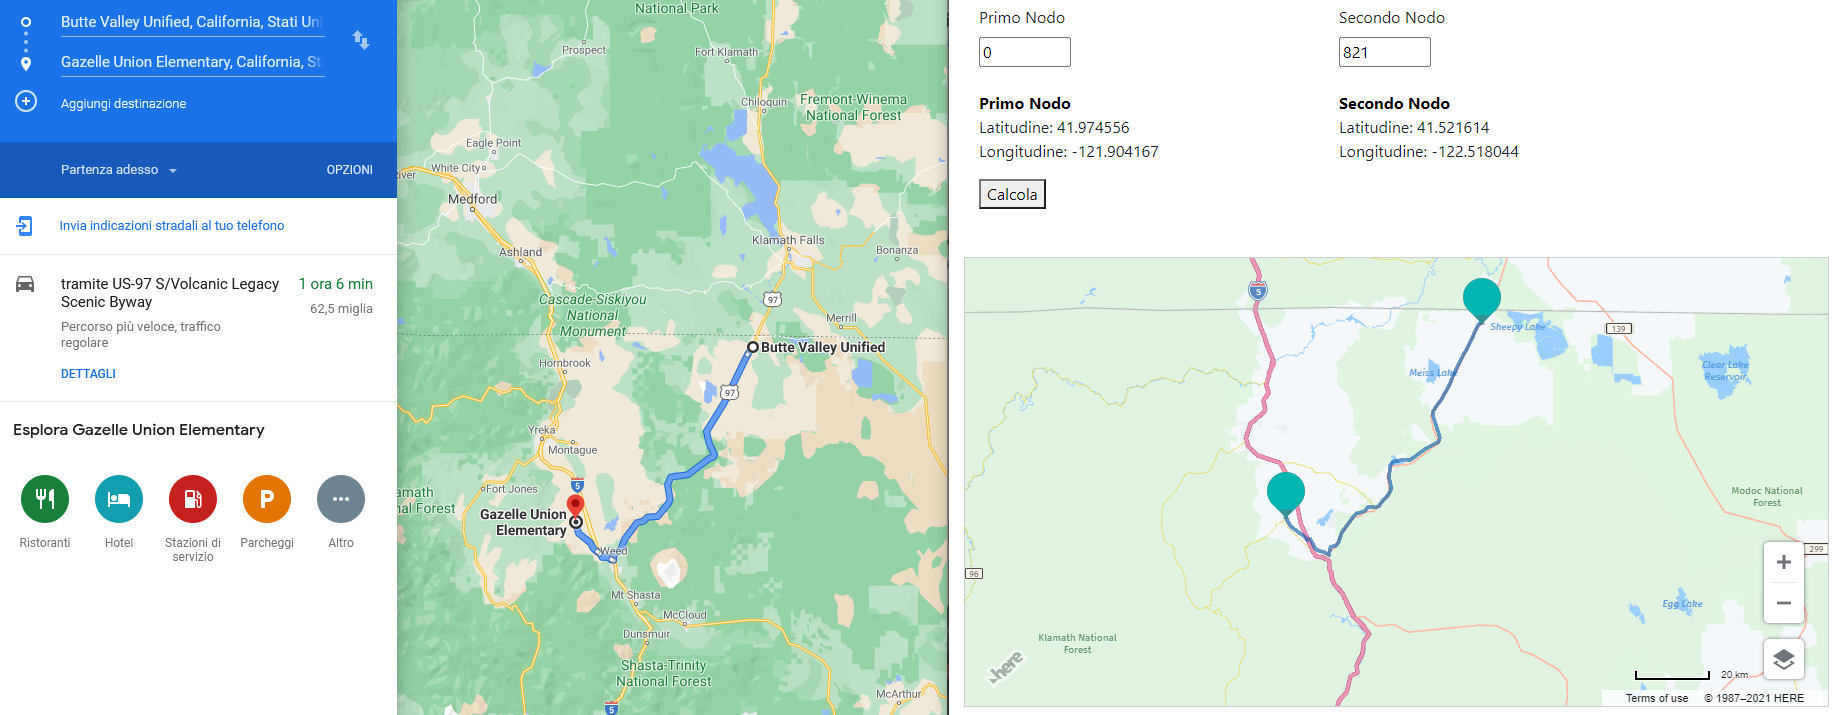
\includegraphics[width=1.05\textwidth]{img/es1.png}
		\caption{Nord della California (con deviazione in Oregon)}
	\end{figure}

	\begin{figure}[H]
		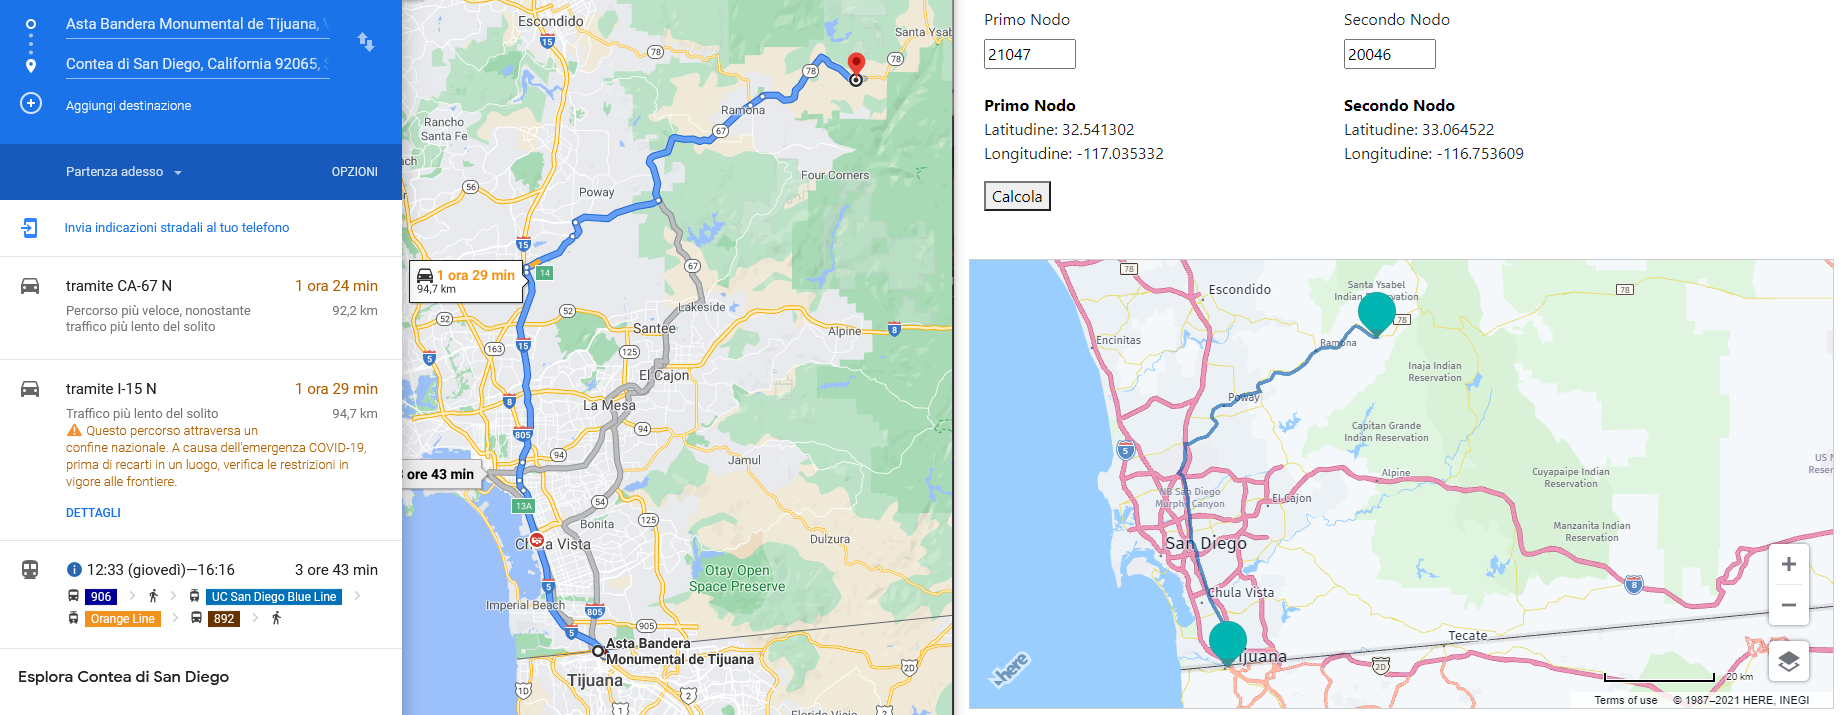
\includegraphics[width=1.05\textwidth]{img/es2.png}
		\caption{Costa Californiana}
	\end{figure}
\bigskip\bigskip\bigskip\bigskip
	\begin{figure}[H]
		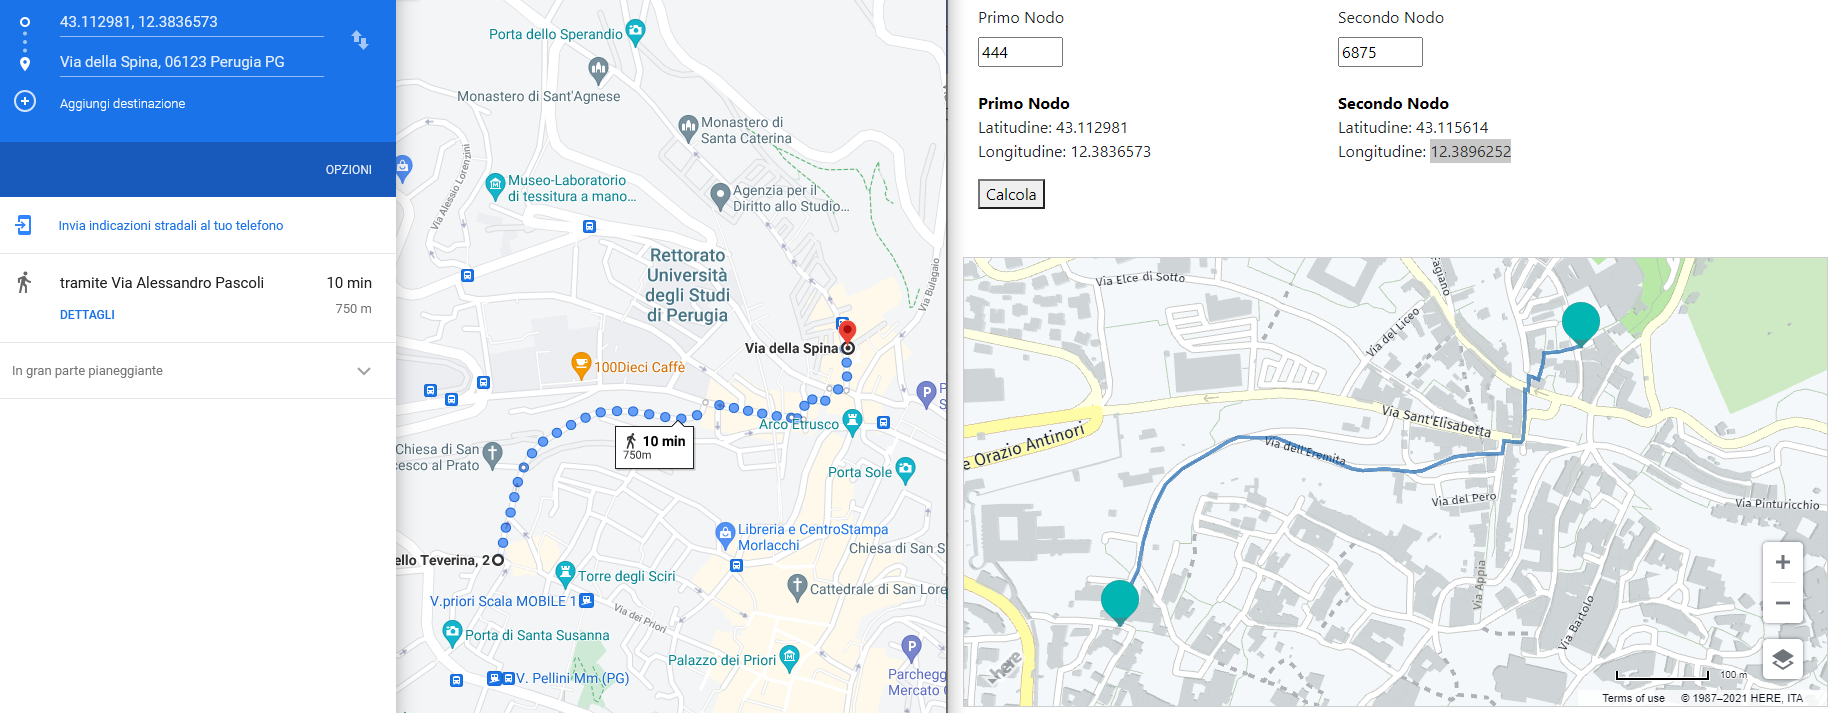
\includegraphics[width=1.05\textwidth]{img/es3.png}
		\caption{Perugia (Nei pressi dell'Università per Stranieri)}
	\end{figure}

	\begin{figure}[H]
		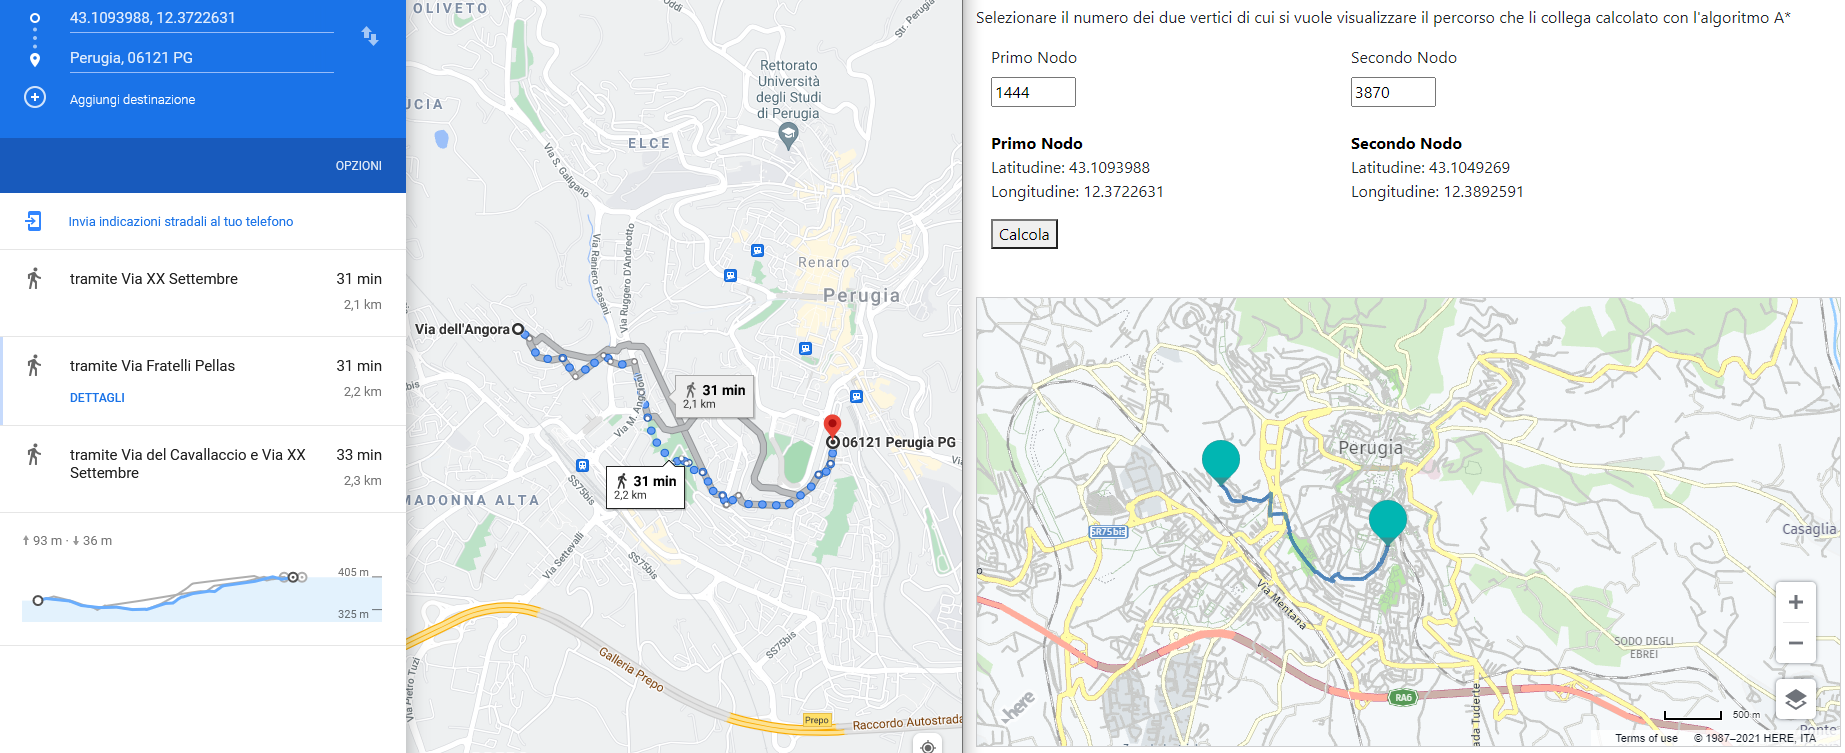
\includegraphics[width=1.05\textwidth]{img/es4.png}
		\caption{Perugia (Nei pressi di Piazza Partigiani)}
	\end{figure}
\end{center}

\chapter{Discussione dei dati\\sperimentali}

Prese coppie di nodi nella mappa stradale della California con fattore di diramazione \(b \simeq N^\frac{1}{d}\), numero totale di vicini N e profondità del cammino ottimo d differenti, abbiamo ricavato la variazione del tempo di esecuzione:

\begin{table}[H]
	\centering
	\begin{tabular}{@{}llll@{}}
		\toprule
		\textbf{d} & \textbf{N} & \textbf{b} & \textbf{Tempo (ms)}       \\ \midrule
		569 & 42695 & 1.0189 & 9  \\
		573 & 42803 & 1.0187 & 12 \\
		577 & 42904 & 1.0186 & 10 \\
		580 & 42964 & 1.0185 & 10 \\ \bottomrule
	\end{tabular}
\end{table}

Abbiamo svolto poi lo stesso lavoro sulla mappa stradale di Perugia ed ottenuto questi risultati:

\begin{table}[H]
	\centering
	\begin{tabular}{@{}llll@{}}
		\toprule
		\textbf{d} & \textbf{N} & \textbf{b} & \textbf{Tempo (ms)}       \\ \midrule
		66  & 6549  & 1.13 & 9  \\
		70  & 6962  & 1.14 & 7  \\
		80  & 9117  & 1.12 & 11 \\
		83  & 9422  & 1.11 & 7  \\
		116 & 13695 & 1.08 & 3 \\ \bottomrule
	\end{tabular}
\end{table}

In entrambe le tabelle si può notare come al crescere di d e di b il tempo di elaborazione effettivamente aumenta. Sperimentalmente abbiamo visto che l'euristica si mantiene buona se b medio è sufficientemente vicino a 1 (\(<\)1.5).

Abbiamo constatato tramite coordinate geografiche reali che effettivamente l'utilizzo di una coda di priorità e dei suoi metodi extractMin(), minHeapify(),
\\insert(), delete() e decreaseKey() il tempo di ricerca del percorso migliore è diminuito nell'ordine dei millisecondi.
Riportiamo di seguito la differenza di tempo d'esecuzione tra A* senza e con code di priorità presi tre tragitti d'esempio (due tra nodi relativamente lontani e l'ultimo tra nodi relativamente vicini).

\begin{table}[H]
	\centering
	\begin{tabular}{@{}llll@{}}
		\toprule
		\textbf{Nodo 1} & \textbf{Nodo 2} & \textbf{Tempo senza PQ (ms)} & \textbf{Tempo con PQ (ms)}\\ \midrule
		7999 & 2231  & 15  & 10  \\
		10000 & 20000  & 25  & 21  \\
		9444 & 9553  & 3  & 2  \\ \bottomrule
	\end{tabular}
\end{table}


\chapter{Fonti}

\begin{itemize}
	\item \href{http://ozark.hendrix.edu/~ferrer/courses/335/f11/lectures/effective-branching.html}{Effective Branching Factor}
	\item \href{http://pages.di.unipi.it/micheli/DID/IIA-2016/part1/4e5-2016-infosearch-post-lez.pdf}{Ricerca Euristica UniPi}
	\item \href{https://www.geeksforgeeks.org/sum-manhattan-distances-pairs-points/}{Manhattan Distance}
	\item \href{https://en.wikipedia.org/wiki/A*_search_algorithm}{A* Serach Algorithm}
	\item \href{https://en.wikipedia.org/wiki/Consistent_heuristic}{Consistent Heuristic}
	\item \href{http://theory.stanford.edu/~amitp/GameProgramming/ImplementationNotes.html}{Game Programming Implementation Notes}
	\item \href{https://www.cs.utah.edu/~lifeifei/SpatialDataset.htm}{Real Datasets for Spatial Databases: Road Networks and Points of Interest}
\end{itemize}



\end{document}